\chapter{Conclusions \& Discussion}\label{discussion}

\epigraph{Your assumptions are your windows on the world. Scrub them off every once in a while, or the light won’t come in.}{Isaac Asimov}

In this final chapter, I summarize the presented work and display my conclusions. In addition, I compare my results with previous studies and provide some estimations about the system's evolution. 

\section{Summary}

In this work, I present one of the few studies of simulating mass transfer in hierarchical triple systems with a focus on RLOF by the tertiary towards the inner binary. 

In the first part, I offer a detailed analysis of the process of creating hydrodynamical models representing a star using \ac{sph} particles, while accounting for its internal structure. In particular, I examine both convective and radiative envelopes, highlighting the various physical mechanisms that must be considered when defining their thermodynamic properties, respectively. In addition, by delving into the details of the relaxation process, I provide useful guidelines for creating stable hydrodynamical models. Finally, I demonstrate the method's efficiency in modeling low- and intermediate-mass stars with convective envelopes, as well as its shortcomings in modeling radiative envelopes, particularly those of massive stars.

In the second part, I describe qualitatively the effect of mass transfer in the evolution of the inner and outer orbits. This is a complicated hydrodynamical problem. The amount of mass and angular momentum that is lost from the system is critical for the system's evolution. Nevertheless, there are nearly no theoretical predictions for the aforementioned quantities. Here, I provide some estimates and qualitative comparisons for two cases: In one case the accretion radii of the inner binary components are slightly smaller than the Roche lobe radii of their initial configuration, see \cref{fig:triple_equop}. In this scenario, I approach the maximal accretion case, effectively setting a lower limit to the amount of lost mass from the system. In the other case, the accretion radii correspond to the physical radii of the binary components, essentially illustrating the scenario of minimal accretion and setting an upper limit to the amount of lost mass from the system. Consequently, I evaluate the importance of the inner binary's accretion efficiency and provide qualitative description of the system's response to the mass transfer in the above cases. Furthermore, I investigate the effect of the initial inclination of the outer orbit relative to the inner orbit, a parameter that is expected to be critical for the mass transfer process. Despite the fact that my simulations' resolution is low, I extract valuable information about the qualitative behavior of the system in these different cases. Finally, I demonstrate that the coupled solver that I deploy can properly capture the intricate three-body dynamics by accommodating the details of Lidov-Kozai cycles. 

The acquired knowledge in hydrodynamically modeling stars, combined with the successful capture of the intricate three-body dynamics, is perhaps the most important indirect result of this work. The code developed for this project is highly adaptable, and minor adjustments allow for the investigation of mass transfer via \ac{rlof} in various triple configurations. For example, the 3D hydrodynamical model could replace one of the inner binary stars effectively simulating \ac{rlof} in the inner binary and also include dynamical perturbations due to an outer star. 



\section{Conclusions}

Mass transfer in hierarchical triple systems, and more particularly, RLOF by the outer star, is different from mass transfer in regular binary systems. The process is fairly complicated, but a qualitative picture is the following: In the presence of a donor with a convective envelope and the absence of a circumbinary disk, mass transfer is expected to be highly non-conservative. As a result, the outer orbit shrinks, while tidal interactions between the inner and outer orbits circularize the latter and push it toward coplanarity with the inner orbit. Given the current resolution, the response of the inner orbit is unclear. The orbit widens for low angles of the incoming mass stream, while shrinks for higher ones. Nonetheless, higher resolution simulations are required to confirm the above trend. Finally, the effect of the mass transfer on the eccentricity of the inner orbit is negligible. However, mutual inclinations well inside the Lidov-Kozai regime result to exchange of angular momentum between the two orbits. The latter appear in the form of periodic variations of the inner eccentricity and the mutual inclination.

The accretion efficiency and the amount of angular momentum carried away by ejected matter are critical for a quantitative description of the process. Assuming that the ejected mass carries a constant amount of specific angular momentum, the lower the accretion efficiency, $\beta$, of the inner binary, the greater the decay of the outer orbit, see \cref{fig:comparison_analytical_model_max}. Consequently, the aforementioned rates of change of orbital parameters are also higher. Such systems are expected become dynamically unstable in shorter timescales. Close encounters and collisions are expected to enhance, which tend to dissolve systems to lower orders \citep{van2007formation}. Systems with higher $\beta$ values are expected to be relatively more stable as less angular momentum is lost during the same time period, see \cref{fig:comparison_analytical_model_max}. The mass transfer is expected to be relatively more stable, at least during the early phase of the process, and to span during longer timescales.

The higher accretion efficiency may also have some observational implications. Because more mass is accreted and also during longer timescales, the inner binary stars can increase their masses and rotational velocities \citep{packet1981rotation}. Consequently, their evolutionary paths may be altered possibly leading to the formation of exotic objects, such as blue strugglers \citep{zwart2019triple}, and/or rapidly rotated binary stars with somehow more homogeneous envelopes \citep{dorozsmai2023stellar}. Furthermore, convective mixing in the deep convective envelope, see \cref{fig:kippen_plot}, brings heavier elements to the donor's surface, see \cref{sec:convection}, and this is the material that is transferred via \ac{rlof}. Hence, effective accretion can also lead to metal-rich binary stars. Even in the case of stellar collisions, the final products will result from now more massive and evolved progenitors. Thus the merger outcome between the two cases (low and high $\beta$) may differ in mass and metallicity. For example, \cite{gao2023stellar} proposed that Barium stars can be formed in hierarchical triples, where \ac{rlof} by the outer star is followed by a merger of the barium rich inner binary components. In conclusion, combining theoretical and observational studies is essential in further constraining $\beta$, $\eta$ and the possible evolutionary outcomes of mass-transferring triples.





\section{Comparison with previous work}

\cite{de2014evolution} simulate the phase of mass transfer for the $\xi$ Tau system using AMUSE. Their study focuses on the effect of the initial mutual inclination on the evolution of the system. Their models include overshooting and they report a type B mass transfer, which is also the case for my models including overshooting. Additionally, they also encounter mass transfer that leads to a common envelope-like structure around the inner binary. Except for the evolution of the inner semi-major axis, the evolution of the outer and inner orbits in my study is qualitatively similar to their results. On the one hand, in \cref{sec:resolution}, I demonstrate that the resolution of my simulations is probably poor, hence this may be a reason behind this discrepancy. On the other hand, \cite{de2014evolution} claim to use the same resolution. Their study covers a larger mass transfer duration, $\sim 40$ yr, but this is expected as in my case the widening of the inner orbit brings the system relatively fast to the unstable regime. In conclusion, my results qualitatively agree with \cite{de2014evolution} study, but higher resolution simulations are needed to confidently conclude about the evolution of the inner semi-major axis during the mass transfer.

In my study, I also investigate the importance of the inner binary's accretion efficiency. The lack of theoretical predictions makes the comparison of the results difficult, but some estimations can be made. In \cite{zwart2019triple} study, the formation of a circumbinary disk leads to accretion efficiency up to $\beta \gtrsim 0.8$, while in my study the model with the highest accretion efficiency corresponds to $\beta = 0.53$, see \cref{fig:inclination_binary_eff}. Keep in mind that, the inner binary in their study has nearly the same size, a comparable period, but smaller accretion radii then my binary components. Despite that, the accretion efficiency is $\sim 30\%$ higher. As a result, it appears that, in the absence of a forming disk, the inner binary rotation makes accretion of incoming mass more difficult since part of it gets ejected via a slingshot effect. In conclusion, the accretion efficiency of the inner binary is most likely strongly related to whether or not a circumbinary disk forms. The absence of a forming disk suggests a highly non-conservative mass transfer. This is an intriguing speculation and an interesting topic for future research.

For the maximal accretion case, I find that a value of $\eta \approx 4$ can describe the evolution of the semi-major axis of the outer orbit, while a value of $\eta \approx 7$ is needed to match the minimal accretion case assuming the same amount of mass is lost. The latter results in a shorter timescale for the process, making these systems more difficult to detect. In comparison, a value of $\eta = 6$ is consistent with non-conservative mass transfer in binaries through the second Lagrangian point \citep{flannery1977origin,portegies1995formation} and it is associated with the formation of a circumbinary ring, see \cref{fig:triple_equop}. Additionally, a value of $\eta \gtrsim 3$ is derived in \cite{portegies1995formation} by matching the orbital evolution and birthrate of Be-type X-ray binaries that experience non-conservative mass transfer. However, values of $\eta = 3-4$ are reported also by \cite{de2014evolution, zwart2019triple} in studies of triples. 

Finally, \cite{zwart2019triple,leigh2020mergers} report that given the formation of a circumbinary disk via \ac{rlof} by the outer star, a preferable accretion towards the less massive binary component occurs. Despite the fact that in my simulations no disk forms, I encounter the same behavior for the models with $i_{mut} \neq 0^{\circ}$, see \cref{fig:inclination_binary_eff}
\begin{figure}[H]
    \centering
    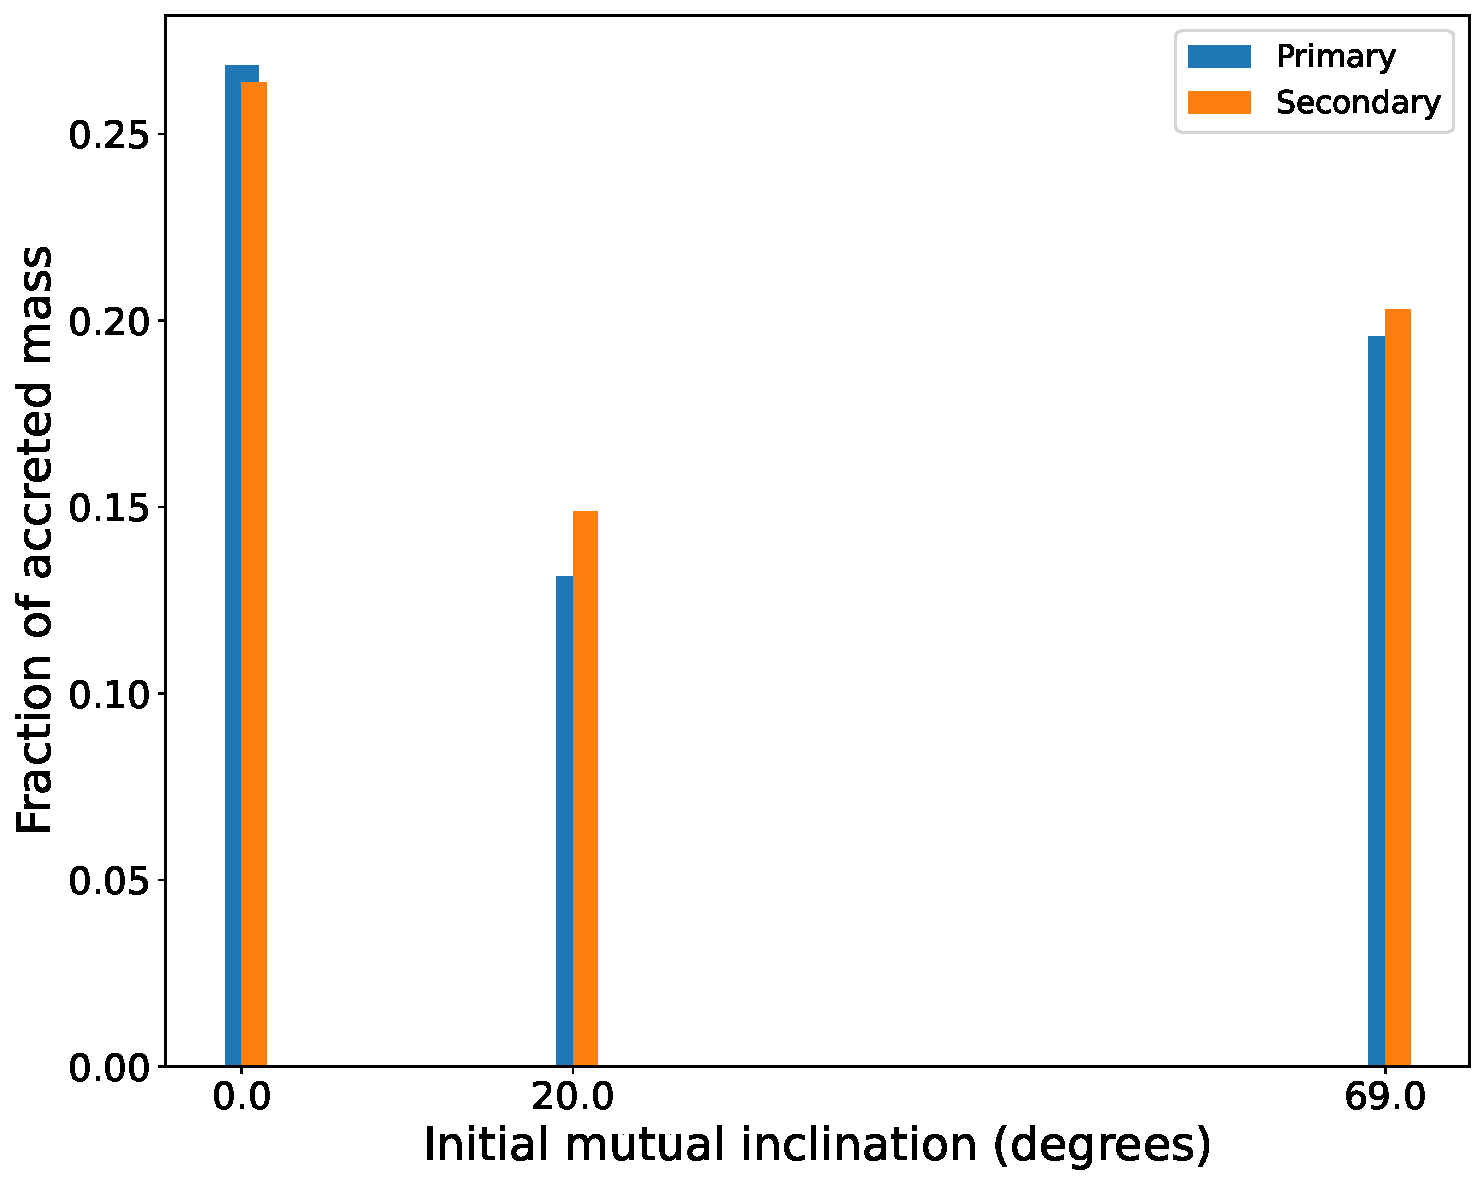
\includegraphics[width=0.9\textwidth]{Thesis/graphs/inclination_case/incliantion_binary_acc_efficiency.pdf}
    \caption{Fraction of the accreted mass by the inner binary stars for different initial inclination of the outer orbit relative to the inner orbit.}
    \label{fig:inclination_binary_eff}
\end{figure}
Quantify distinct trends in \cref{fig:inclination_binary_eff} is not trivial, due to the complicated transport of mass, angular momentum and energy between the outer star, and the accretion stream onto the individual inner stars. More importantly, running higher resolution simulations before trying to interpret this result is necessary. Because gas drag may alter the details of the accretion process. Nonetheless, this outcome is interesting to be investigated due to the fact that it hints towards a mechanism of producing equal mass binaries. 


\section{Future of $\xi$ Tau}\label{sec:discussion}

It is not easy to predict the system's future. One critical parameter is the donor star's reaction to mass-loss. On the one hand, the reduction of the donor's mass shrink its Roche lobe. On the other hand, the donor is a red giant with a deep convective envelope. The convective envelope ensures that the radius of the giant remains constant or even expands adiabatically due to mass loss during the early stage of the process, see Onno Pols `Binary Stars`. At the same time, the outer orbit becomes circular and coplanar with the inner orbit. As a result, a continuous and accelerated mass-loss in a circular orbit, initially replaces the current picture of periodic mass-loss. To draw conclusions about later stages, detailed calculations of the donor's Roche lobe and adiabatic response to mass-loss are required. If the donor's adiabatic response is unable to keep it within its Roche lobe, the result is an ever-increasing mass-transfer rate, resulting in dynamically unstable mass transfer. In the opposite case, after significant mass-loss, the donor will react adiabatically and detach from its Roche lobe. The radius will continue to expand on a thermal timescale until \ac{rlof} is re-established, resulting in a thermal-timescale mass transfer, which is self-regulated.

The second critical parameter is the response of the inner orbit. If the inner orbit truly expands, the system enters the unstable regime, see \cref{eq:stability_regime}, and most likely will dissolve to a lower order via collision or ejection of one star. If the inner orbit shrinks, though, the ratio between the semi-major axes' rate of change,
\begin{equation}
    \frac{\dot{a_{in}}/a_{in}}{\dot{a_{out}/a_{out}}},
\end{equation}
determines the system's future. In this case, the system shrinks as a whole and if the ratio is close to unity, the system remains dynamically stable. Furthermore, if $\dot{a_{in}}/a_{in}$ is significant enough, the system will enter in a new phase of \ac{rlof} initiating in the inner binary, and thus a new cycle of interesting triple evolution will take place. Despite, the multiple scenarios, observations of hierarchical triple systems with white dwarfs orbiting close \ac{ms} binaries, where both orbits are circular and on the same plane, would be attractive candidates for the evolutionary scenario outlined in this work.

\begin{comment}
    

For complicity, I mention that in the aforementioned case where the system remains dynamically stable and the inner binary accretes matter some extra parameters needs to be considered. These are the response of the binary components to the accretion. Accretion is likely to spin-up the accreting stars to high rotational velocities \citep{packet1981rotation} setting an upper limit to their individual accretion efficiency.


The evolution of binary systems during mass transfer can be quite complicated, and the addition of a third star adds to the process's complexity. The late type B case of \ac{rlof} by an outer star toward an inner binary presented here is short-lived, probably occurring on the donor's thermal timescale, $\Delta t \approx t_{th}$, or on $t_{dyn} \leq \Delta t \leq t_{th}$. Hence, direct observational counterparts are expected to be extremely rare.  However, considering the implications of the accretion efficiency and angular momentum loss some further theoretical estimations can be made. 

On the one hand, low values of $\beta$ should be connected with more unstable systems. As angular momentum is lost rapidly, the fraction of the inner and outer orbit changes in shorter timescales, see \cref{eq:stability_regime}. Hence, such systems enter the unstable regime in shorter timescales. Close encounters and collisions are expected to enhance, which tend to dissolve systems to lower orders \citep{van2007formation}. On the other hand, higher values of $\beta$ are connected with more stable systems as less amount of angular momentum is lost assuming the same $\eta$, see \cref{fig:comparison_analytical_model_max}. The mass transfer is expected to be somehow more stable and to occur during longer timescales. The higher accretion efficiency of material during longer timescales allow the inner binary stars to increase their masses and rotational velocities. The latter will impact their evolutionary paths and can possibly lead to the formation of exotic objects, such as blue strugglers, and/or rapidly rotated stars with somehow more homogeneous envelopes. 

More specifically, peculiar observed systems could possibly reveal insights regarding their progenitors 


\subsection{Future work}

The evolution of binary systems during mass transfer can be quite complicated, and the addition of a third star adds to the process's complexity. Additional constraints on the accretion efficiency and angular momentum loss are critical in order to better understand the evolution and the outcome of these systems. First, it is important to repeat the simulations with higher resolution in order to verify the observed trends and the calculated values for $\beta$ and $\eta$. 
\end{comment}












\begin{comment}
    


In this case, the angular momentum vectors of the inner binary and the inflowing gas are (almost) aligned, hence less angular momentum is required to accelerate the gas to the escape velocity. Furthermore, on the current resolution the gas drag is considerably underestimated.

Indeed, when the angular momentum vectors of the inner binary and the inflowing gas are (almost) aligned, less angular momentum needs to be transferred to speed up the gas to the escape velocity.


s.

The work is partially exploratory, as I try to test the efficiency of the method considering different internal structure for the donor star.


I use AMUSE \citep{pelupessy2013astrophysical,portegies2018astrophysical} in order to handle stellar evolution, hydrodynamics and gravity in a self-consistent way.




\section{Discussion}

In this section, I describe some crucial features of the modeling method that will assist the reader in interpreting the graphs, presented in the next sections. 
\end{comment}